Para realizar el experimento, simplemente debe ejecutar el archivo datasets.py y este le generara los 6 datasets, luego simplemente debe ejecutar el archivo main.cpp, este le generar un archivo csv con los tiempos de ejecucion, estos datos los pasa a un excel para generar el gráfico.

% Dataset 1
\section{Resultados Experimentales}

A continuación, se presentan los gráficos generados para los diferentes conjuntos de datos utilizados en la experimentación.

\begin{enumerate}
    \item \textbf{Dataset1}: 
    \begin{figure}[H]
        \centering
        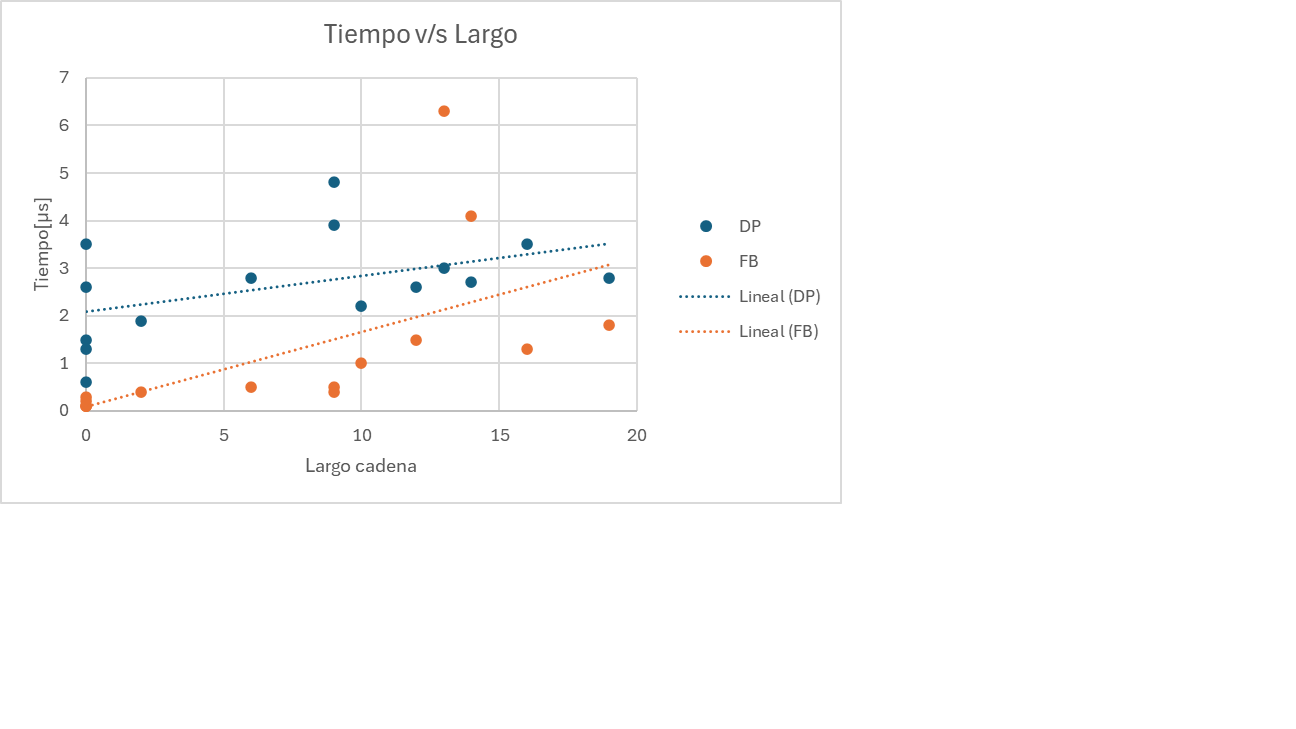
\includegraphics[width=\textwidth]{tikz/Grafico1.png}
        \caption{Gráfico correspondiente a Dataset1. Cadenas vacías.}
        \label{fig:dataset1}
    \end{figure}

    \item \textbf{Dataset2}: 
    \begin{figure}[H]
        \centering
        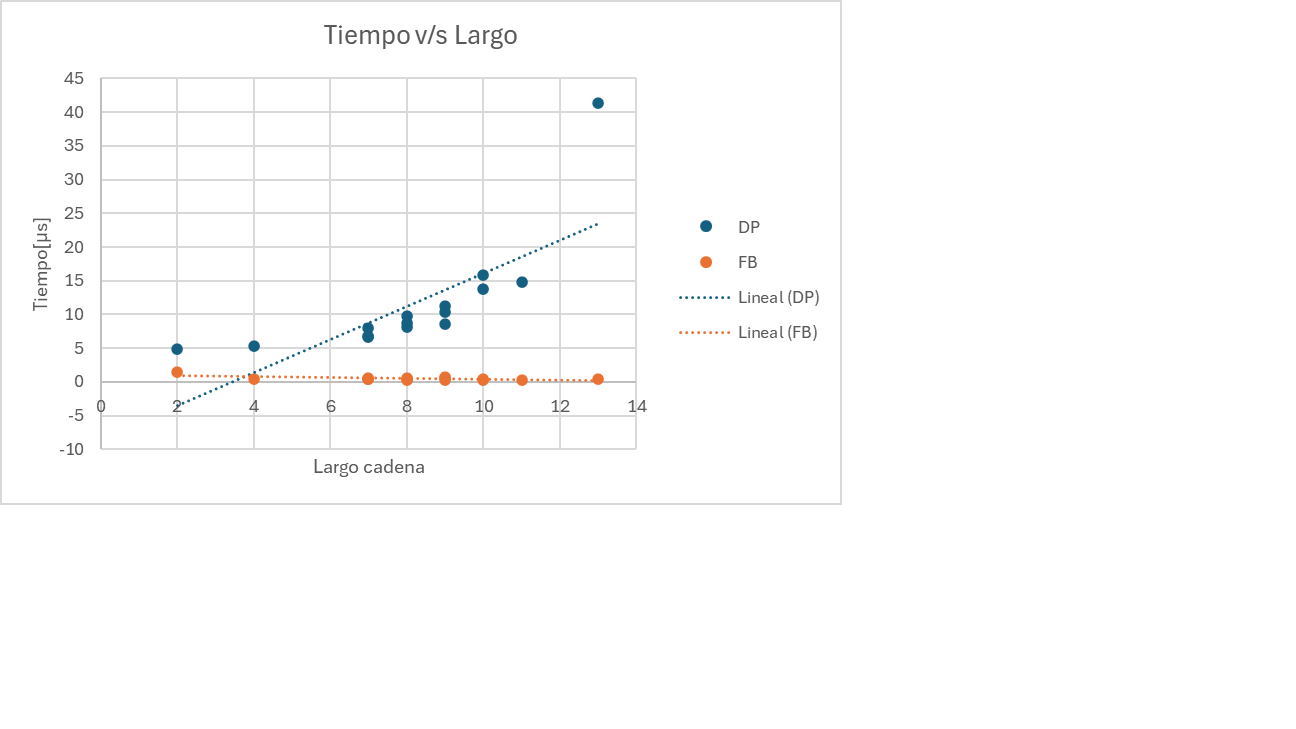
\includegraphics[width=\textwidth]{tikz/Grafico2.png}
        \caption{Gráfico correspondiente a Dataset2. Cadenas identicas.}
        \label{fig:dataset2}
    \end{figure}

    \item \textbf{Dataset3}: 
    \begin{figure}[H]
        \centering
        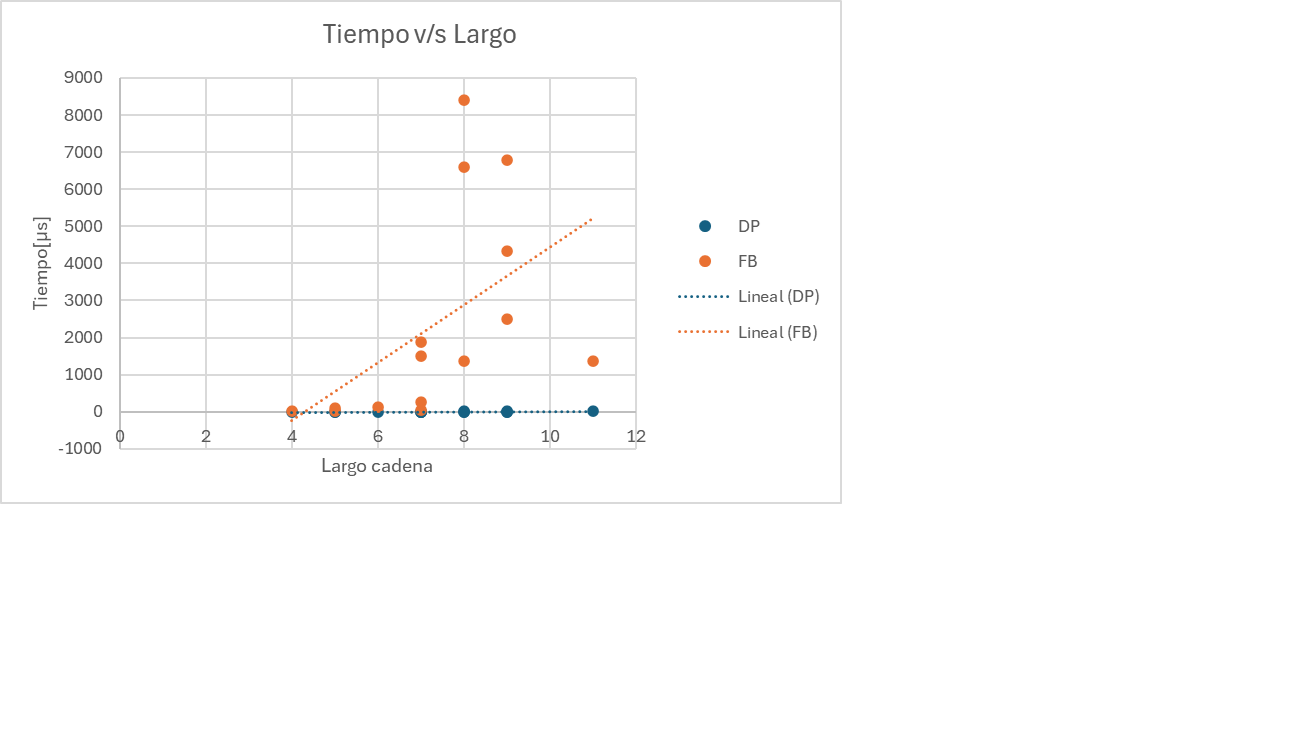
\includegraphics[width=\textwidth]{tikz/Grafico3.png}
        \caption{Gráfico correspondiente a Dataset3. Cadenas con caracteres repetidos.}
        \label{fig:dataset3}
    \end{figure}

    \item \textbf{Dataset4}: 
    \begin{figure}[H]
        \centering
        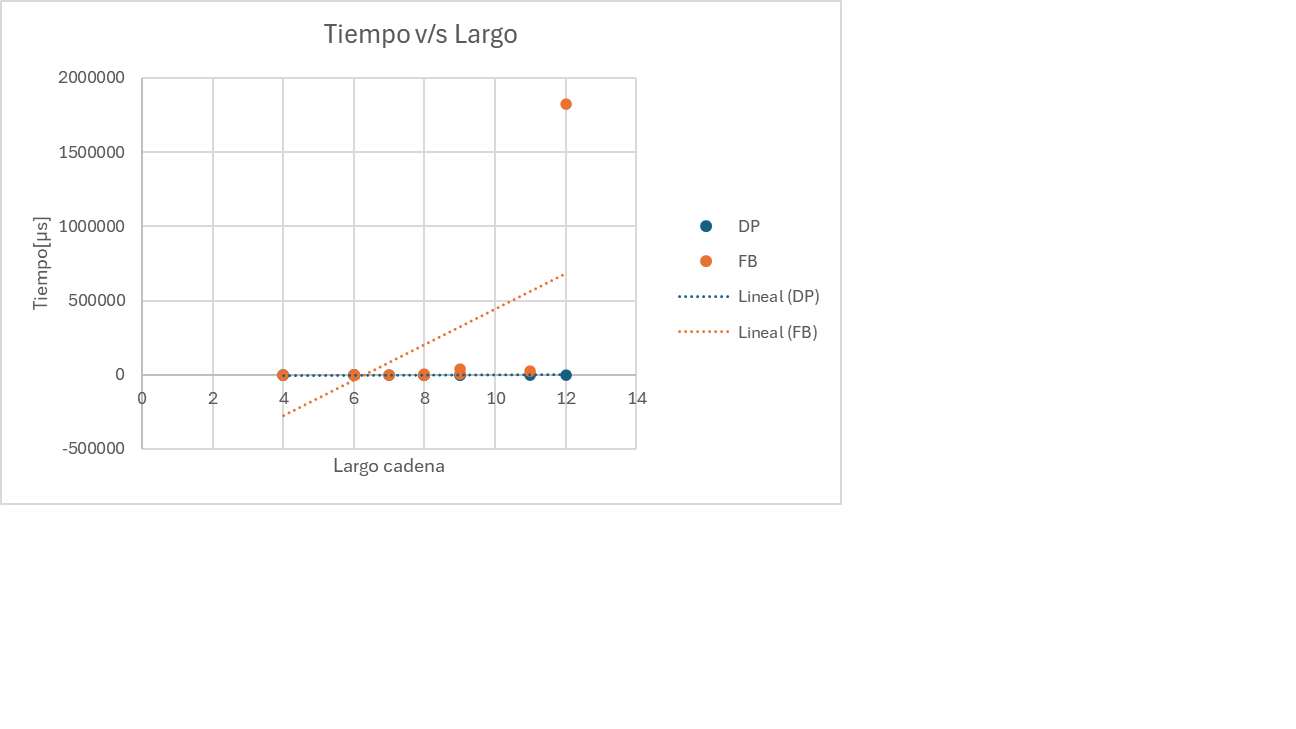
\includegraphics[width=\textwidth]{tikz/Grafico4.png}
        \caption{Gráfico correspondiente a Dataset4. Cadenas aleatorias con mismo tamaño.}
        \label{fig:dataset4}
    \end{figure}

    \item \textbf{Dataset5}: 
    \begin{figure}[H]
        \centering
        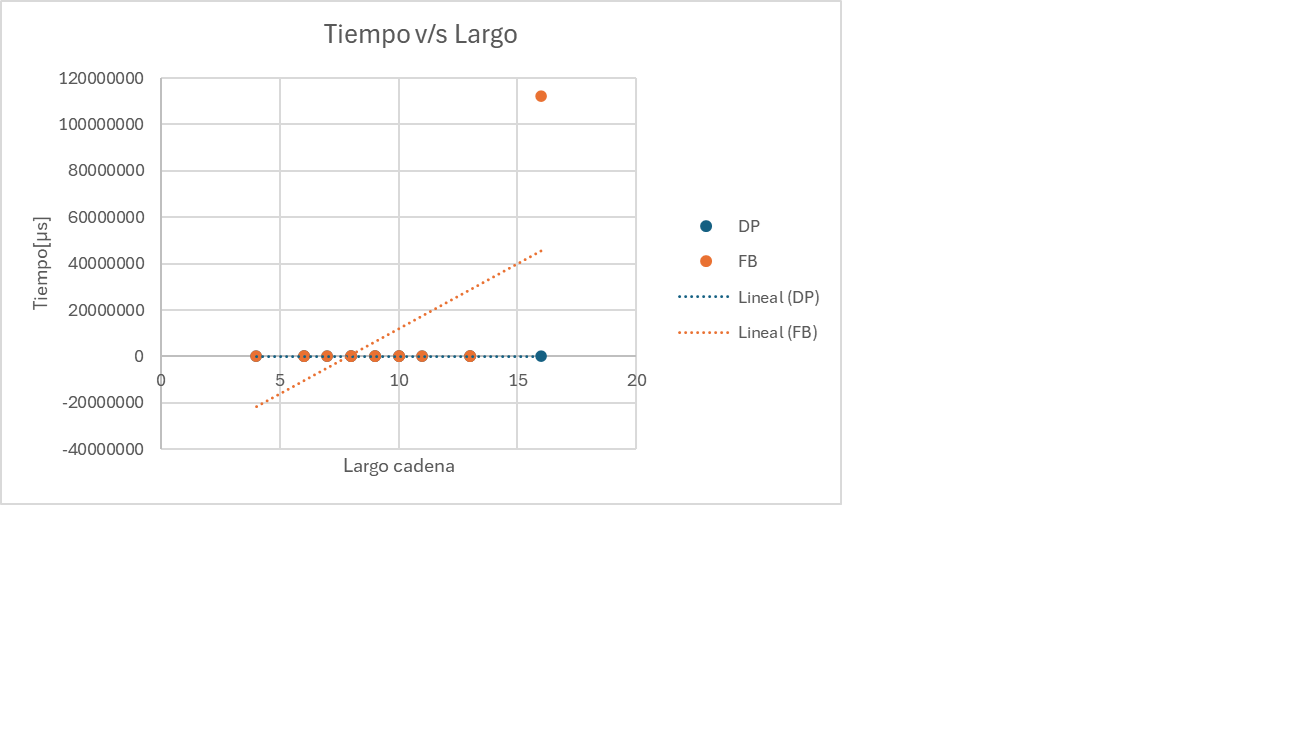
\includegraphics[width=\textwidth]{tikz/Grafico5.png}
        \caption{Gráfico correspondiente a Dataset5. Cadenas aleatorias con diferentes tamaños.}
        \label{fig:dataset5}
    \end{figure}

    \item \textbf{Dataset6}: 
    \begin{figure}[H]
        \centering
        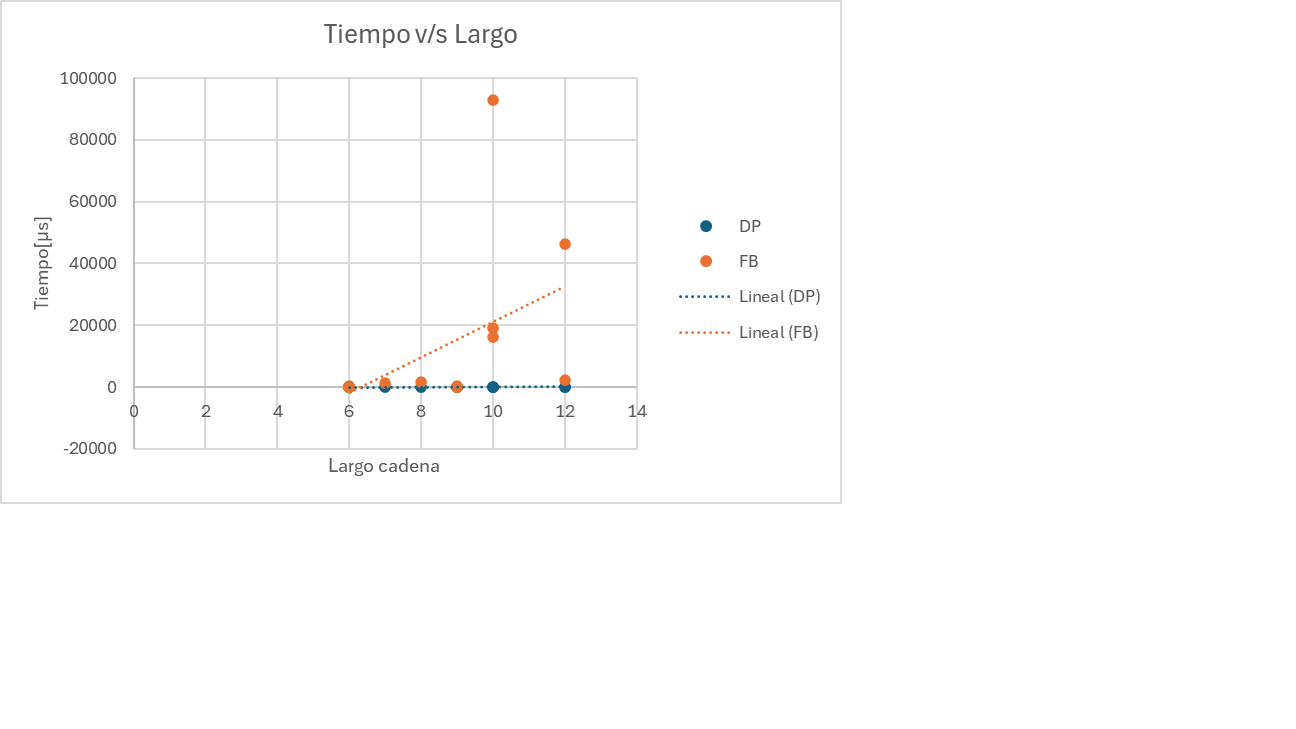
\includegraphics[width=\textwidth]{tikz/Grafico6.png}
        \caption{Gráfico correspondiente a Dataset6. cadenas con transposiciones.}
        \label{fig:dataset6}
    \end{figure}
\end{enumerate}
